\section{Stellar Consensus Protocol}
\subsection{Nomination Protocol}

Nomination is done through voting, accepting, and confirming a special type of statement in the form of \textit{nominate $x$}.

\begin{defn}[Nomination Statement]
    \textit{nominate $x$} is a special statement which is short for
    \begin{itemize}
        \item
            \textit{Value $x$ passes application validity checks, and}
        \item
            \textit{I have never confirmed a nomination statement}.
    \end{itemize}
\end{defn}

\begin{defn}[Nominate]
    A node is said to nominate a value $x$ if and only if it votes for the statement \textit{nominate $x$} before any other node.
\end{defn}

\begin{defn}[Renominate]
    A node is said to renominate a value $x$ if and only if it votes for the statement \textit{nominate $x$} after some other node votes for it.
\end{defn}

\begin{defn}[Candidate]
    A node $v$ considers a value $x$ to be a candidate if and only if $v$ has confirmed the statement \textit{nominate $x$}.
    Alternatively, we say that $v$ has a candidate value $x$.
\end{defn}

\begin{defn}[Produce]
    A node is said to produce a candidate value $x$ when it confirms \textit{nominate $x$} after nominating it.
\end{defn}

\begin{rem}
    This approach is slightly different from the white paper's.
    The white paper seems to define some special ``rule" on voting for a nomination statement.
    However, that seems to change the definition of voting (Definition~\ref{def_vote}), and I was unable to convince myself that we could simply apply FBA arguments after changing the definition of voting.
    On the other hand, we defined a nomination statement to be a statement containing some special instructions.
    This approach should achieve the same thing while utilizing the fact that a well-behaved node is allowed to vote for a valid statement that is consistent with history.
\end{rem}

\begin{thm}\label{eventually_one_candidate}
    The set of intact nodes will eventually produce at least one candidate value.
\end{thm}

The white paper mentions that the set of intact nodes \textit{can} eventually produce at least one candidate value.
However, we should be able to change it to \textit{will} as long as nodes without candidate values continue renominating other candidate's values.

\begin{proof}
    Suppose that, at some point in time, an intact node confirms a nominate statement.
    Then we are done.
    Suppose otherwise.

    Let $v$ be an intact node and $x$ be a value that passes application validity checks.
    We assume that $v$ is capable of finding such a value.
    Then $v$ will vote for \textit{nominate $x$}.
    By Definition \ref{defn_network}, the message will eventually get delivered to all intact nodes.
    Since the value passes application validity checks and no intact node has confirmed a nominate statement, every intact node will eventually vote for \textit{nominate $x$}.
    By the definition of a DSet(Definition~\ref{def_dset}), the set of all intact nodes is a quorum, so all the intact nodes will accept and confirm \textit{nominate $x$} after sufficient messages have been delivered.
    This is a contradiction because we assumed that no intact node confirms a nominate statement.

    Therefore, the set of intact nodes can eventually produce at least one candidate value.
\end{proof}

\begin{lem}\label{intact_cannot_accept_no_vote}
    In an FBAS that enjoys quorum intersection, an intact node cannot accept a statement that no intact node voted for.
\end{lem}

We will use this lemma to prove Theorem~\ref{nomination_property_1}.

\begin{proof}
    On the contrary, suppose that it is possible.
    Let $x$ be a statement that no intact node voted for and $v$ be the first intact node that accepts it.

    In order for an intact node $v$ to accept $x$, we need
    \begin{itemize}
        \item
            The existence of a quorum $U$ containing $v$ such that every member of $U$ either voted for or accepted $x$, or
        \item
            A $v$-blocking set consisting of nodes that accepted $x$.
    \end{itemize}

    However, neither of them is possible because
    \begin{itemize}
        \item
            We assumed that no intact node ever voted for $x$.
            Therefore, $v$ never voted for $x$.
            Thus the first condition can never be satisfied.
        \item
            Let $B$ be such a $v$-blocking set.
            The set of intact nodes is a quorum by Corollary~\ref{set_of_intact_nodes_quorum}.
            Therefore, $B$ must contain at least one intact node $w$.
            However, this implies that $w$ accepted $x$ before $v$.
            This is a contradiction because we specifically picked $v$ such that $v$ is the first node to accept the statement.
            Therefore, the second condition can never be satisfied.
    \end{itemize}

    Therefore, it is impossible for $v$ to accept $x$.
\end{proof}

\begin{thm}\label{nomination_property_1}
    If an FBAS enjoys quorum intersection, the set of possible candidate values eventually stops growing.
\end{thm}

\begin{proof}
    By Theorem~\ref{eventually_one_candidate}, at least one intact node will confirm \textit{nominate $x$} for some $x$.
    By Theorem~\ref{all_intact_nodes_accept_confirm_same_things}, all intact nodes will confirm it.
    Therefore, there exists a point $T$ in time where all intact nodes have at least one candidate value.

    Let $S$ denote the set of all nomination statements that intact nodes voted for before $T$.
    $S$ is finite because $T$ is a specific point in time.

    We claim that $S$ is the set of possible candidate values, and a nomination statement outside $S$ can never be confirmed.

    We will first show that a nomination statement outside $S$ cannot be accepted by an intact node.
    No intact node will ever vote for a nomination statement after $T$.
    Therefore, $S$ is the set of all nomination statements that intact nodes will ever vote for.
    By Lemma~\ref{intact_cannot_accept_no_vote}, no intact node will ever accept a statement not in $S$.

    The set of intact nodes is a quorum by Corollary~\ref{set_of_intact_nodes_quorum}.
    Since the FBAS enjoys quorum intersection, any quorum intersects the set of intact nodes.
    In other words, any quorum contains an intact node.
    Therefore, it is impossible for any quorum to confirm a statement not in $S$.
    Hence, $S$ is the set of possible candidate values.
\end{proof}

\todo[inline,caption={}]{
    prove the third property
}

\todo[inline,caption={}]{
    prove theorem 12
}


\begin{defn}[Weight, Neighbors, and Priority]
    Let $H$ be a cryptographic hash function whose range can be interpreted as a set of integers $\{ 0, \cdots, h_{\max} - 1 \}$.
    Let $G_i(m) = H(i, x_{i - 1}, m)$ be a slot-specific hash function for slot $i$, where $x_{i - 1}$ is the value chosen for the slot preceding $i$.
    Let $N \ne P$ are arbitrary constants.
    Given a slot $i$, a round number $n$ and node $v$, we define
    \begin{align*}
        \weight(v, v') &= \frac{\abs{\{ q \in Q(v) \mid v' \in q \}}}{\abs{Q(v)}} \\
        \neighbors(v, n) &= \{ v' \mid G_i(N, n, v') < h_{\max} \cdot \weight(v, v') \} \\
        \priority(n, v') &= G_i(P, n, v')
    \end{align*}
    for each neighbor $v'$.
\end{defn}

\begin{rem}
    In Stellar Core, $N$ and $P$ are always $1$ and $2$.
\end{rem}

\begin{defn}[Leader]
    Let a slot $i$, round number $n$, and node $v$ be given.
    Then the node $v_0 \in \neighbors(v, n)$ that maximizes $\priority(n, v_0)$ among the nodes it can communicate with is considered to be the leader by $v$.
    Node $v$ votes to nominate the same values as $v_0$.
    Only if $v = v_0$, $v$ can introduce a new value to nominate.
\end{defn}

\begin{exmp}[Weight, Neighbors, and Priority]
    We will calculate the weight, neighbors, and priority for $v_5$ in Figure~\ref{fig:tiered_quorum_example} as an example.
    Since each quorum slice consists of $v_5$ along with two nodes from $\{ v_1, v_2, v_3, v_4 \}$ as in
    \begin{align*}
        Q(v_5) &= \{ \{ v_1, v_2, v_5 \}, \{ v_1, v_3, v_5 \}, \{ v_1, v_4, v_5 \}, \cdots, \{ v_3, v_4, v_5 \} \},
    \end{align*}
    $Q(v_5)$ has $\binom{4}{2} = 6$ slices.

    We will first calculate the weight of $v_1$.
    \begin{align*}
        \weight(v_5, v_1)
            &= \frac{\abs{\{ q \in Q(v_5) \mid v_1 \in q \}}}{\abs{Q(v_5)}} \\
            &= \frac{\abs{ \{ v_1, v_2, v_5 \}, \{ v_1, v_3, v_5 \}, \{ v_1, v_4, v_5 \}}}{6} \\
            &= \frac{3}{6} = \frac{1}{2}.
    \end{align*}
    By symmetry, $\weight(v_5, v_j) = \frac{1}{2}$ for each $j = 1, 2, 3, 4$.
    $\weight(v_5, v_5) = 1$ because every quorum slice in $Q(v_5)$ contains $v_5$.
    Finally, $\weight(v_5, v_j) = 0$ for all $j = 6, 7, 8, 9, 10$ because no quorum slice in $Q(v_5)$ contains any of $v_6, v_7, \cdots, v_{10}$.
    Therefore, we obtain the following table:
    \begin{center}
      \begin{tabular}{ | c | c | }
        \hline
          $j$ & $\weight(v_5, v_j)$ \\ \hline
          1, 2, 3, 4 & $\nicefrac{1}{2}$ \\ \hline 
          5 & 1 \\ \hline 
          6, 7, 8, 9, 10 & 0 \\
        \hline
      \end{tabular}
    \end{center}

    For this example, we will suppose that $h_{max} = 100$.
    Let $N, P, i, n$ be fixed.
    Then we will calculate the neighbors.
    First, we will start with $v_1, v_2, v_3, v_4$.

    Suppose
    \begin{align*}
        G_i(N, n, v_1) &= 41 \\
        G_i(N, n, v_2) &= 72 \\
        G_i(N, n, v_3) &= 19 \\
        G_i(N, n, v_4) &= 84.
    \end{align*}
    The condition for a node $v'$ to be in $\neighbors(v_5, n)$ is $G_i(N, n, v') < 100 \cdot \weight(v_5, v')$.
    Therefore, $v_1, v_3 \in \neighbors(v_5, n)$.
    (e.g., $G_i(N, n, v_1) = 41 < 50 = 100 \cdot 1/2 = 100 \cdot \weight(v_5, v_1)$.)

    Moreover, $v_5 \in \neighbors(v_5, n)$ since $\weight(v_5, v_5) = 1$.
    Finally, $v_j \in \neighbors(v_5, n)$ for each $j = 6, 7, \cdots, 10$ because $\weight(v_5, v_j) = 0$.

    Therefore, we have
    \begin{align*}
        \neighbors(v_5, n) = \{ v_1, v_3, v_5 \}.
    \end{align*}
    This is a reasonable choice of neighbors because
    \begin{itemize}
        \item
            $v_5$ trusts $v_1, \cdots, v_4$, so it is a good thing that we have $v_1, v_3$ in $\neighbors(v_5, n)$.
        \item
            $v_5$ trusts $v_5$.
        \item
            Since $v_5$ does not trust $v_6, \cdots, v_{10}$, $v_5$ has no quorum slice containing any of them.
            Thus it is a good thing that $\neighbors(v_5, n)$ does not contain any of them.
    \end{itemize}

    Finally, suppose
    \begin{align*}
        \priority(n, v_1) &= G_i(P, n, v_1) = 17 \\
        \priority(n, v_3) &= G_i(P, n, v_3) = 86 \\
        \priority(n, v_5) &= G_i(P, n, v_5) = 25.
    \end{align*}

    Then $v_5$ will simply nominate the same value as $v_3$.
\end{exmp}

\begin{rem}
    $ $
    \begin{itemize}
        \item
            $\weight$ is not symmetric in general.
            In other words, $\weight(v_i, v_j) \ne \weight(v_j, v_i)$ in general.
        \item
            $\neighbors(v_i)$ is a set of nodes calculated locally at each $v_i$.
            In general, $\neighbors(v_i) \ne \neighbors(v_j)$ for any $i \ne j$.
        \item
            $\priority(n, v)$ is \textit{global} in a sense that the values of $\priority(n, v)$ calculated at node $w$ and $w'$ must be identical for it only depends on $n$, the hash function $G_i$ and the constant $P$.
    \end{itemize}
\end{rem}

\begin{exmp}[Leader Election]
    We will again use the FBAS in Figure~\ref{fig:tiered_quorum_example} as an example.
    Suppose that each node's neighbors is as follows:
    \begin{center}
      \begin{tabular}{ | c | c | }
        \hline
            $j$ & $\neighbors(v_j)$ \\ \hline
            1 & $\{ v_1, v_3 \}$ \\ \hline
            2 & $\{ v_2, v_4 \}$ \\ \hline
            3 & $\{ v_2, v_3, v_4 \}$ \\ \hline
            4 & $\{ v_1, v_2, v_4 \}$ \\ \hline
            5 & $\{ v_2, v_5 \}$ \\ \hline
            6 & $\{ v_1, v_3, v_6\}$ \\ \hline
            7 & $\{ v_1, v_2, v_3, v_7 \}$ \\ \hline
            8 & $\{ v_3, v_8 \}$ \\ \hline
            9 & $\{ v_6, v_7, v_8, v_9 \}$ \\ \hline
            10 & $\{ v_{10} \}$ \\
        \hline
      \end{tabular}
    \end{center}
    Suppose that $\priority(n, v_j) = G_i(P, n, v_j)$ for each $j$ is as follows:
    \begin{center}
      \begin{tabular}{ | c | c | c | c | c | c | c | c | c | c | c | }
        \hline
            $j$ & 1 & 2 & 3 & 4 & 5 & 6 & 7 & 8 & 9 & 10 \\ \hline
            $\priority(n, v_j)$ &  26 & 3 & 60 & 89 & 18 & 56 & 35 & 19 & 61 & 27\\
        \hline
      \end{tabular}
    \end{center}
    Note that the priority of each node is \textit{global}.
    For instance, $\priority(n, v_1)$ calculated at $v_2$ and $v_6$ are the same.
    Thus it makes sense to have a table like this.

    Then each node's leader (the node whose nominations it will renominate) will be as follows:
    \begin{center}
      \begin{tabular}{ | c | c | c | c | c | c | c | c | c | c | c | }
        \hline
            $j$ & 1 & 2 & 3 & 4 & 5 & 6 & 7 & 8 & 9 & 10 \\ \hline
            $v_j$'s leader & $v_3$ & $v_4$ & $v_4$ & $v_4$ & $v_5$ & $v_3$ & $v_3$ & $v_3$ & $v_9$ & $v_{10}$ \\
        \hline
      \end{tabular}
    \end{center}

    \begin{figure}[!htb]
        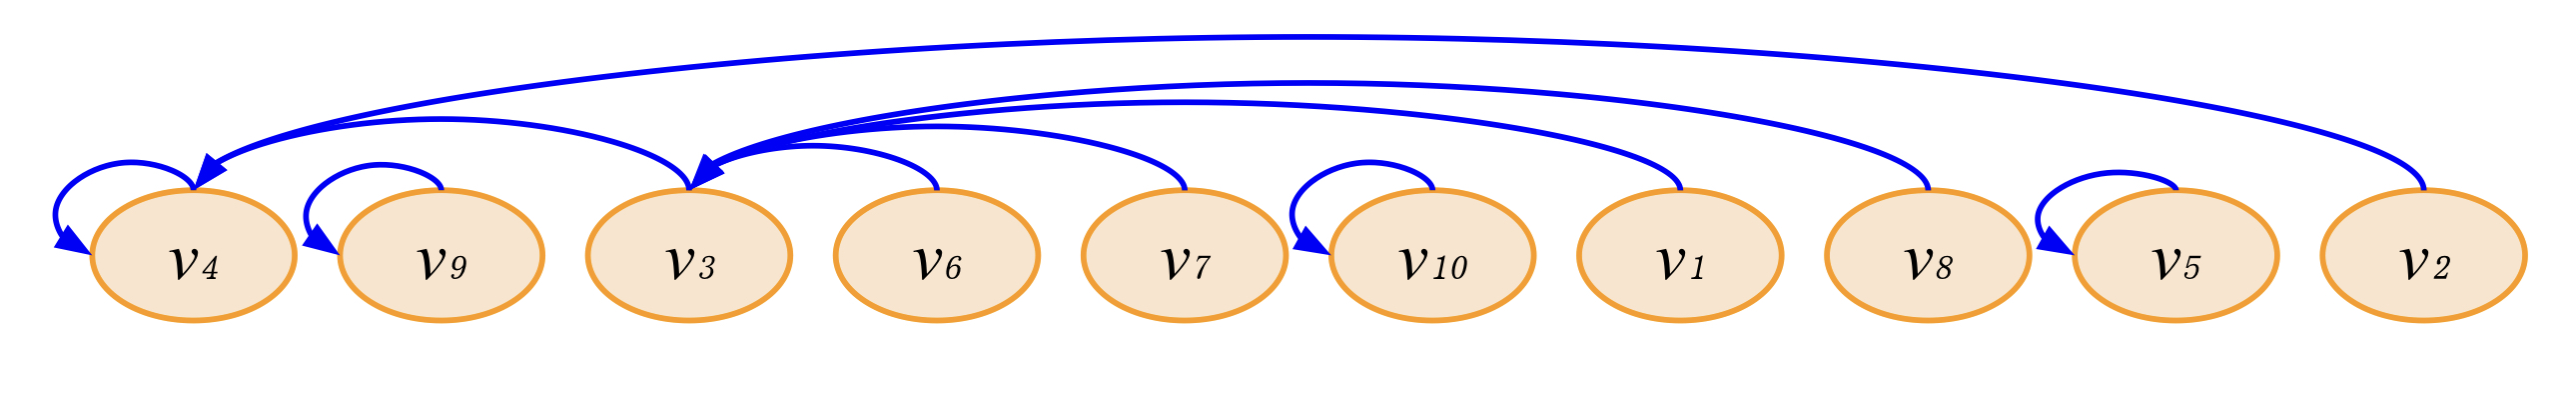
\includegraphics[width=.8\linewidth]{img/leader_election.jpeg}
        \caption{Leader Relation Graph}
        \label{fig:leader_relation}
    \end{figure}

    As you can see, this is a directed graph such that the only cycles are self-loops.
    In this particular case, $v_4, v_9, v_{10}, v_5$ will produce new values, and other nodes will simply renominate those values.
\end{exmp}

\begin{exmp}[Leader Election With A Failed Node]
    Suppose that, in the previous example, node $v_3$ stops responding due to a power outage.
    Since the leader is the node in the neighbors that maximizes the priority among the nodes that it can communicate with, no node will pick $v_3$ as their leader.
    Under this circumstance, each node will pick the following nodes as their leader:

    \begin{center}
      \begin{tabular}{ | c | c | c | c | c | c | c | c | c | c | c | }
        \hline
            $j$ & 1 & 2 & 3 & 4 & 5 & 6 & 7 & 8 & 9 & 10 \\ \hline
            $v_j$'s leader & $v_3$ & $v_4$ & $v_4$ & $v_4$ & $v_5$ & $v_3$ & $v_3$ & $v_3$ & $v_9$ & $v_{10}$ \\
        \hline
      \end{tabular}
    \end{center}

    \begin{figure}[!htb]
        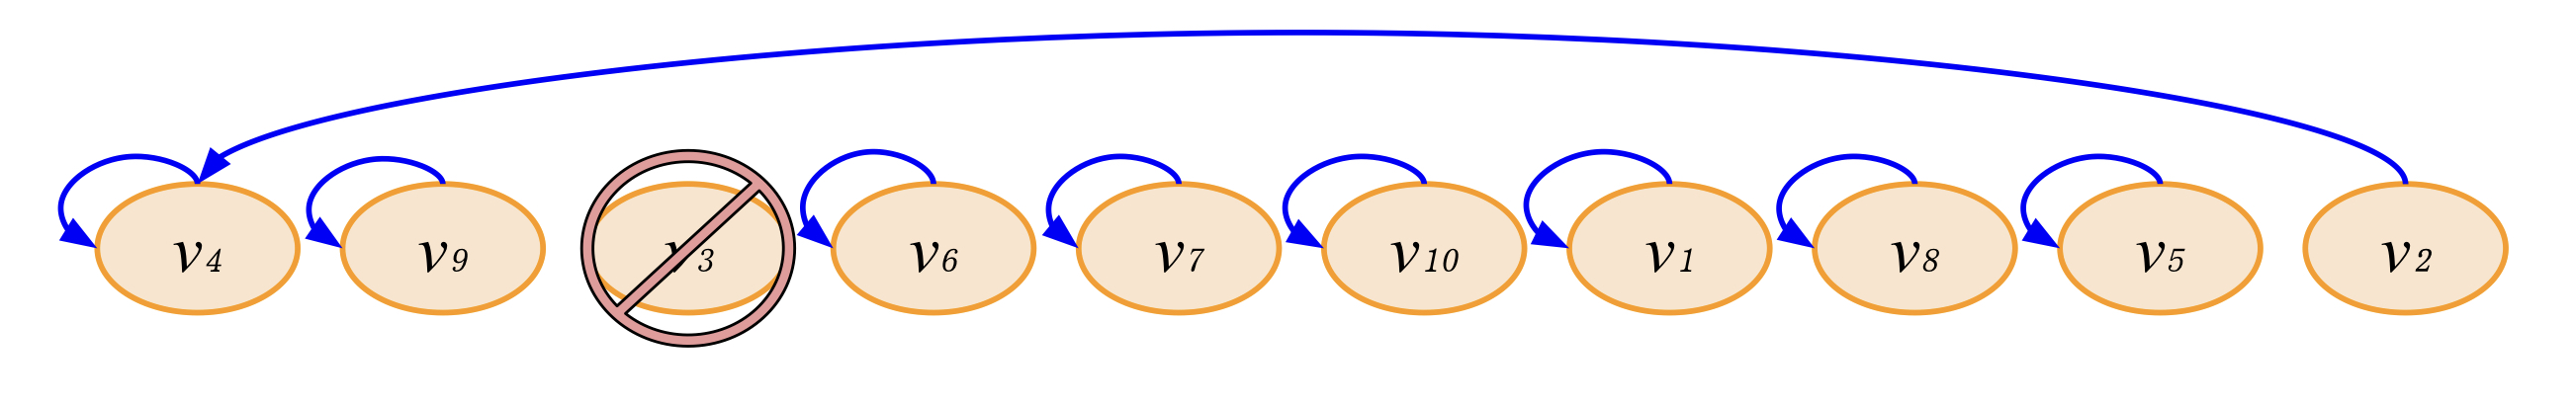
\includegraphics[width=.8\linewidth]{img/leader_election_with_failed_node.jpeg}
        \caption{Leader Relation Graph}
        \label{fig:leader_relation_with_failed_node}
    \end{figure}
    
    In this case, all the nodes except for $v_3, v_2$ will produce new values while $v_2$ will simply renominate the what $v_4$ votes for.
\end{exmp}

\newpage
\subsection{Ballot Protocol}

\begin{defn}[Ballot]
    A ballot $b$ is a pair of the form $b = \ev{n, x}$ where $x \ne \bot$ is a value and $n \geq 1$ is a counter.
\end{defn}

\begin{defn}[Order]
    For any ballots $b_1, b_2$, $b_1 \leq b_2$ if and only if $(b_1.n, b_1.x) \leq (b_2.n, b_2.x)$ in dictionary order.
\end{defn}

\begin{defn}[Null ballot]
    $\textbf{0} = \ev{0, \bot}$ is a special null invalid ballot that is less than any other ballots.
\end{defn}

\begin{defn}[Compatability]
    For a pair of ballots $b_1, b_2$, we define $\sim, \nsim, \lesssim, \lnsim$ as following:
    \begin{align*}
        b_1 \sim b_2 &\iff b_1.x = b_2.x \\
        b_1 \nsim b_2 &\iff b_1.x \ne b_2.x \\
        b_1 \lesssim b_2 &\iff b_1 \leq b_2 \land b_1 \sim b_2 \\
        b_1 \lnsim b_2 &\iff b_1 \leq b_2 \land b_1 \nsim b_2.
    \end{align*}
\end{defn}

\begin{defn}[Commit]
    For a given ballot $b$, \textit{commit} $b$ is a shorthand for ``I have confirmed \textoverline{\textit{commit} $b'$} for all $b' \lnsim b$."
\end{defn}

\textoverline{\textit{commit} $b'$} denotes a statement that contradicts \textit{commit} $b'$.

\begin{rem}[Abort]
    For a given ballot $b$, we will often write \textit{abort} $b$ instead of \textoverline{\textit{commit} $b$} for readability.
\end{rem}

\begin{exmp}
    Let $a, b, c, d, e$ be statements.
    The following table shows what statements a node needs to confirm to abort before \textit{commit} $(3, c)$:
    \begin{center}
        \begin{tabular}{|c|c|c|c|c|c|}
            \hline
            $(n, x)$ & $x = a$        & $x = b$        & $x = c$ & $x = d$        & $x = e$        \\ \hline
            $n = 1$  & \textit{abort} & \textit{abort} &         & \textit{abort} & \textit{abort} \\ \hline
            $n = 2$  & \textit{abort} & \textit{abort} &         & \textit{abort} & \textit{abort} \\ \hline
            $n = 3$  & \textit{abort} & \textit{abort} &         & \textit{abort} & \textit{abort} \\ \hline
            $n = 4$  &                &                &         &                &                \\ \hline
        \end{tabular}
    \end{center}

    Note that
    \begin{itemize}
        \item
            $(2, c)$ is \textit{not} $\lnsim (3, c)$ because they have the same value.
        \item
            $(3, a) \lnsim (3, c)$ because $3 \leq 3$ and $a \ne c$.
    \end{itemize}
\end{exmp}

\begin{defn}[Prepare]
    Let $b$ be a ballot.
    A node is said to vote, accept, or confirm that \textit{$b$ is prepared} if and only if it votes, accepts, or confirms \textit{abort} $b'$ for all $b' \lnsim b$, respectively.
\end{defn}

\begin{rem}
    By the definition of committing and preparing, a node can vote for \textit{commit} $b$ if and only if it has confirmed that $b$ is prepared.
\end{rem}

\begin{rem}
    The approach presented here is slightly different from the white paper's approach.
    In the white paper, the fact that \textit{commit} $b$ is valid to vote for only if $b$ is confirmed prepared is a (seemingly arbitrary) ``rule."
    However, I was not very convinced by this approach because it would mean that we are changing the definition of voting.
    More specifically, the definition of voting states that one votes for a statement \textit{if and only if} the four conditions have been met.  
    However, this new ``rule" will prevent a node from voting even when the four conditions have been met in some cases.

    In the approach presented above, the ``rule" is embedded in the commit statement itself.
    Therefore, there is no need to change the ``rule" around voting.
\end{rem}

\begin{defn}[Externalize]
    A node \textit{externalizes} a value $x$ if and only if it confirms \textit{commit} $\ev{n, x}$ for some $n \geq 1$.
\end{defn}
